% The Higgs boson is produced through four main production mechanisms at the LHC\@: gluon-gluon fusion (ggF), vector boson fusion (VBF), associated production with a vector boson (VH) and top fusion (ttH). The feynman diagrams for the production modes can be seen in Figure~\ref{fig:higgs_production_modes}, while Figure~\ref{fig:higgs_production_function_of_com} illustrates the production cross sections as a function of the $\sqrt{s}$ for each production mode. The dominant Higgs boson production mode at the LHC is ggF. This is followed by VBF which is an order of magnitude smaller. In the same order of magnitude is VH (Higgstrahlung), where WH has a higher cross section than ZH\@. Finally, there is ttH/bbH production which are of the same order of magnitude as ZH.

The Higgs boson is produced at the LHC primarily through four mechanisms: gluon-gluon fusion (ggF), vector boson fusion (VBF), associated production with a vector boson (VH), and associated production with top/bottom quarks (ttH/bbH). Feynman diagrams for these production modes are shown in Figure~\ref{fig:higgs_production_modes}, while Figure~\ref{fig:higgs_production_function_of_com} displays their production cross sections as functions of $\sqrt{s}$. 

\begin{figure}[pht]
  \centering
  \subfloat[Feynman diagrams for the main Higgs boson production modes. Taken from~\cite{Higgs_production_diagrams}\label{fig:higgs_production_modes}]{
    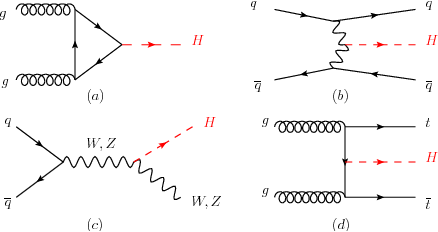
\includegraphics[width=0.55\textwidth]{figures/theory/theory_higgs_prod_feynman.png}
  }
  \hspace{0.01\textwidth}
  \subfloat[Higgs boson production cross sections as a function of $\sqrt{s}$ for the different production modes, taken from~\cite{LHC_Higgs_handbook}.\label{fig:higgs_production_function_of_com}]{
    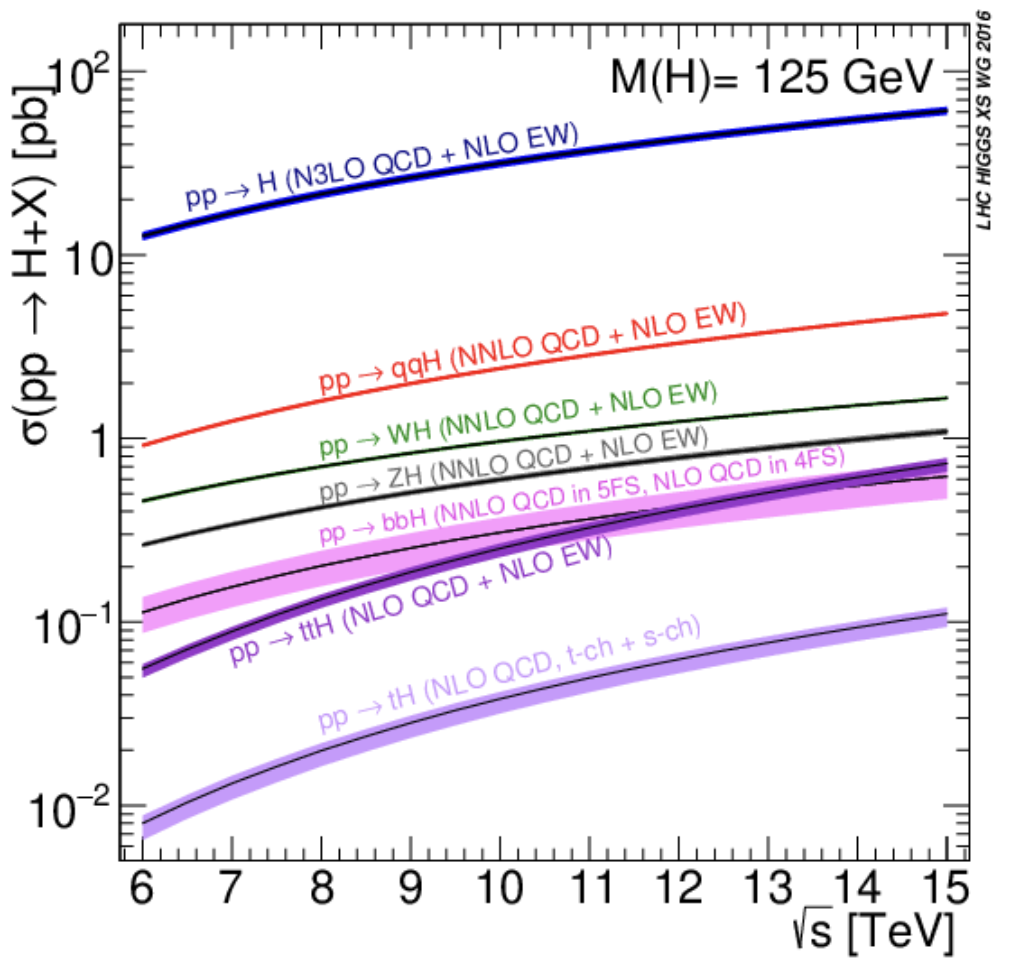
\includegraphics[width=0.35\textwidth]{figures/theory/theory_production_xs.png}
  }
  \caption{Higgs boson production mechanisms and cross sections at the LHC.}
\end{figure}

Of these, ggF ($pp \rightarrow H$) is the dominant production mechanism. Although the Higgs boson does not couple directly to gluons since they are massless, it can be produced via a loop of virtual quarks. This loop is predominantly mediated by top quarks since the Higgs boson couples to fermions with a strength proportional to their mass. The top quark is by far the heaviest known fermion, so it has the largest contribution to the ggF process.

VBF ($pp \rightarrow qqH$) follows with a cross section about an order of magnitude smaller. In this process a quark from each proton emit a $W^{\pm}$ or $Z$ boson that fuse to produce a Higgs boson. The resulting final state is characterized by two high energy forward jets. 

The VH (Higgstrahlung) process ($pp \rightarrow WH$ and $pp \rightarrow ZH$) occurs with a similar cross section to VBF\@. In these events quarks from colliding protons fuse into a vector boson, which then radiates a Higgs boson. $WH$ production occurs is more common than $ZH$ due to the the presence of two $W$ bosons and one $Z$ boson. 

Finally, ttH/bbH production ($pp \rightarrow t\bar{t}H$ and $pp \rightarrow b\bar{b}H$) are of the same order of magnitude as $ZH$. These events occur when gluons from each colliding proton decay into a $t\bar{t} \slash b\bar{b}$ pair, and then one $t \slash b$ from each proton fuse into a Higgs boson leaving a final state with two top/bottom quarks and a Higgs boson. 

For this thesis, the production mode of interest is the $VH$ production mode with a focus on the $WH$ channel. Table~\ref{tab:higgs_production_cross_sections} summarizes the production cross sections for each mechanism at $\sqrt{s} = 13$ TeV.

\begin{table}
  \centering
  \begin{tabular}{c|c}
    \hline
    Production Mode & Cross Section (pb) \\
    \hline
    ggF & $52.23^{+3.79}_{-4.69}$ \\
    VBF & $4.078^{+0.12}_{-0.12}$ \\
    $WH$ & $1.457^{+0.04}_{-0.04}$ \\
    $ZH$ & $0.9439^{+0.01}_{-0.01}$ \\
    $t\bar{t}H$ & $0.57^{+0.04}_{-0.06}$ \\
    $b\bar{b}H$ & $0.5266^{+0.11}_{-0.14}$ \\
    \hline
  \end{tabular}
  \caption{Higgs boson production cross sections at $\sqrt{s} = 13.6$ TeV for the different production modes, taken from~\cite{Higgs_production_cross_sections}.}\label{tab:higgs_production_cross_sections}
\end{table}

% \begin{figure}[pht]
%   \centering
%   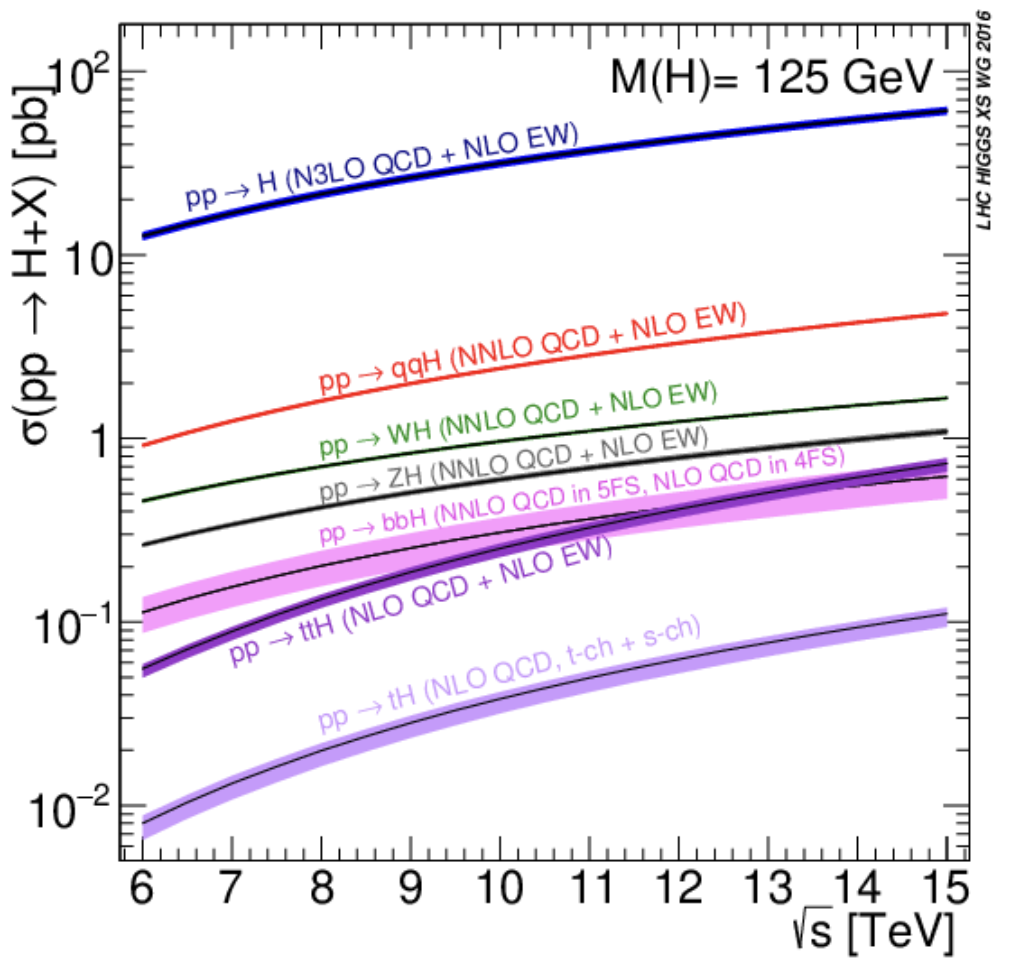
\includegraphics[width=0.6\textwidth]{figures/theory/theory_production_xs.png}
%   \caption{Higgs boson production cross sections as a function of $\sqrt{s}$ for the different production modes, taken from~\cite{LHC_Higgs_handbook}.}\label{fig:higgs_production_function_of_com}
% \end{figure}